%%******************************************************************************
%%
%% nomenclatura.tex
%%
%%******************************************************************************
%%
%% Title......: Nomenclatura
%%
%% Author.....: GSCAR-DFKI
%%
%% Started....: Nov 2013
%%
%% Emails.....: renan028@gmail.com
%%
%% Address....: Universidade Federal do Rio de Janeiro
%%              Caixa Postal 68.504, CEP: 21.945-970
%%              Rio de Janeiro, RJ - Brasil.
%%
%%******************************************************************************


%%******************************************************************************
%% CHAPTER - Nomenclatura
%%******************************************************************************
\section{Nomenclatura}
\begin{itemize}

\item \emph{Stoplog}: Bloco de aço com vinte metros de comprimento, três metros
de altura e três metros de largura (20x3x3 m). O fluxo de água do rio é
controlado pelo empilhamento de \emph{Stoplogs} (figura~\ref{nomenclatura_1} ).


\item \emph{Lifting Beam}: Estrutura mecânica responsável pelo deslocamento de
\emph{Stoplogs}, composta por: duas garras não atuadas, duas chaves de operação, vigas e mecanismo. Um guindaste atua neste mecanismo (figura~\ref{nomenclatura_2}).
    
\item \emph{Guindaste}: O guindaste é capaz de sustentar todo o conjunto
\emph{Lifting Beam}/\emph{Stoplog} e é atuado por um motor elétrico
(figura~\ref{nomenclatura_3} ).

\item \emph{Garra pescadora}: Garra localizada no \emph{Lifting Beam} que se
prende ao \emph{Stoplog}. O mecanismo é composto por duas garras (figura~\ref{nomenclatura_4} ).

\item \emph{Chave de operação}: Localizada na viga principal, próxima à garra
pescadora, seleciona o modo de operação.  Atuada manualmente (figura~\ref{nomenclatura_5} ).

\item \emph{Olhal}: Grande ilhó localizado na parte supeior do \emph{Stoplog}
utilizado como ponto de encaixe para a \emph{Garra pescadora}
(figura~\ref{nomenclatura_6} ).

\end{itemize}

\begin{figure}[H]
    \centering
    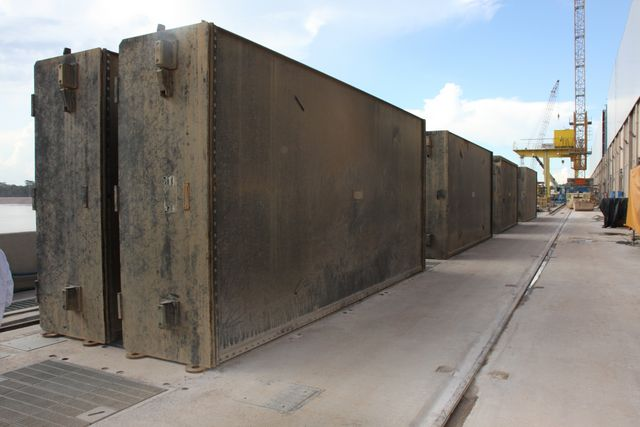
\includegraphics[width=1\columnwidth]{figs/nomenclatura/1.jpg}
    \caption{Stoplogs.}
    \label{nomenclatura_1}
\end{figure}

\begin{figure}[H]
    \centering
    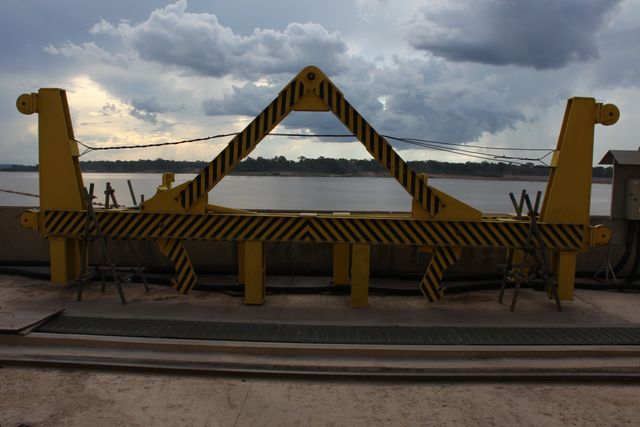
\includegraphics[width=1\columnwidth]{figs/nomenclatura/2.jpg}
    \caption{\emph{Lifting Beam}.}
    \label{nomenclatura_2}
\end{figure}

\begin{figure}[H]
    \centering
    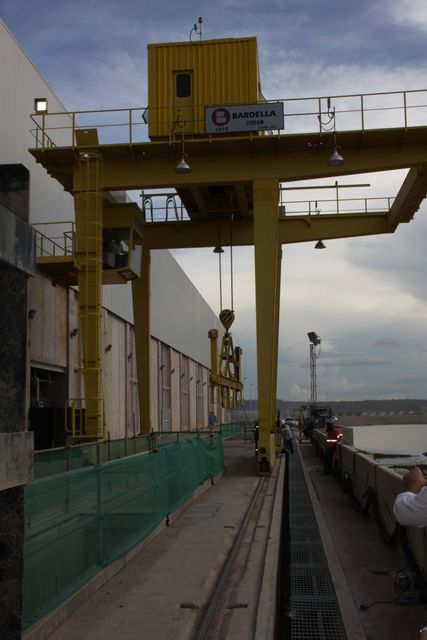
\includegraphics[width=1\columnwidth]{figs/nomenclatura/3.jpg}
    \caption{\emph{Guindaste}.}
    \label{nomenclatura_3}
\end{figure}

\begin{figure}[H]
    \centering
    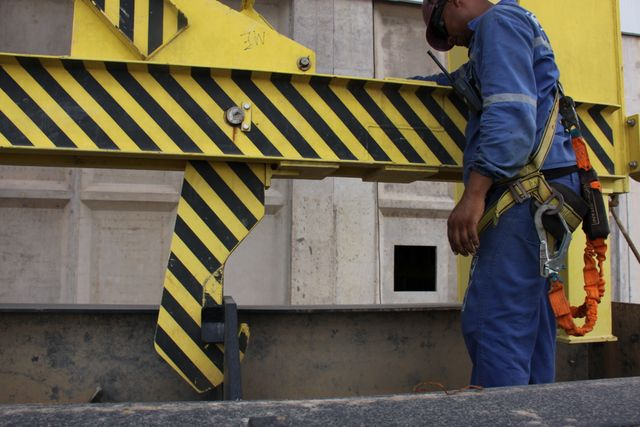
\includegraphics[width=1\columnwidth]{figs/nomenclatura/4.jpg}
    \caption{\emph{Garra pescadora}.}
    \label{nomenclatura_4}
\end{figure}

\begin{figure}[H]
    \centering
    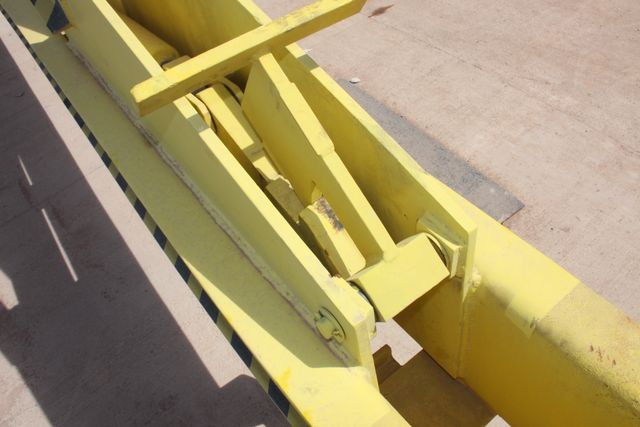
\includegraphics[width=1\columnwidth]{figs/nomenclatura/5.jpg}
    \caption{\emph{Chave de operação}.}
    \label{nomenclatura_5}
\end{figure}

\begin{figure}[H]
    \centering
    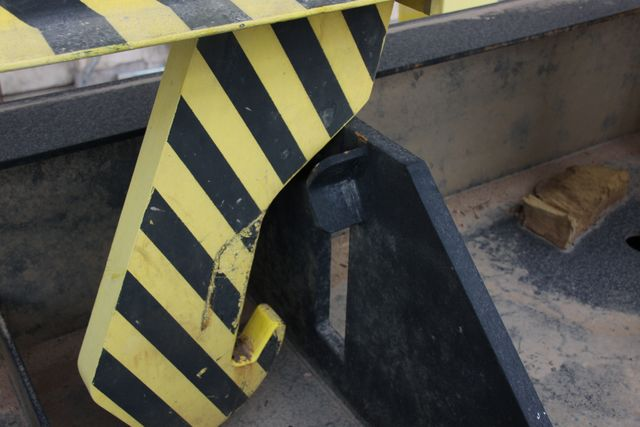
\includegraphics[width=1\columnwidth]{figs/nomenclatura/nomenclatura_6.jpg}
    \caption{\emph{Olhal}.}
    \label{nomenclatura_6}
\end{figure}
